

\section{Introduction}\label{sec:intro}


Input embedding layers in language models map discrete tokens to continuous vector representations~\citep{mikolov2013efficient, sennrich2015neural} before passing them to the subsequent layers. Since tokens are typically simple integer values, the mapping can be implemented purely as memory fetch operations with no additional computation needed.
This allows embedding layers to be offloaded from the limited accelerator memory to main memory or even to secondary storage, such as solid-state drives, with minimal impact on inference speed. This is highly desirable, as main memory and secondary storage are significantly more cost-effective than accelerator memory (e.g., GPUs and TPUs)~\citep{memory_disk_price}. These advantages motivate us to explore methods for scaling up embedding layers.


\begin{figure*}[ht]
    \centering
    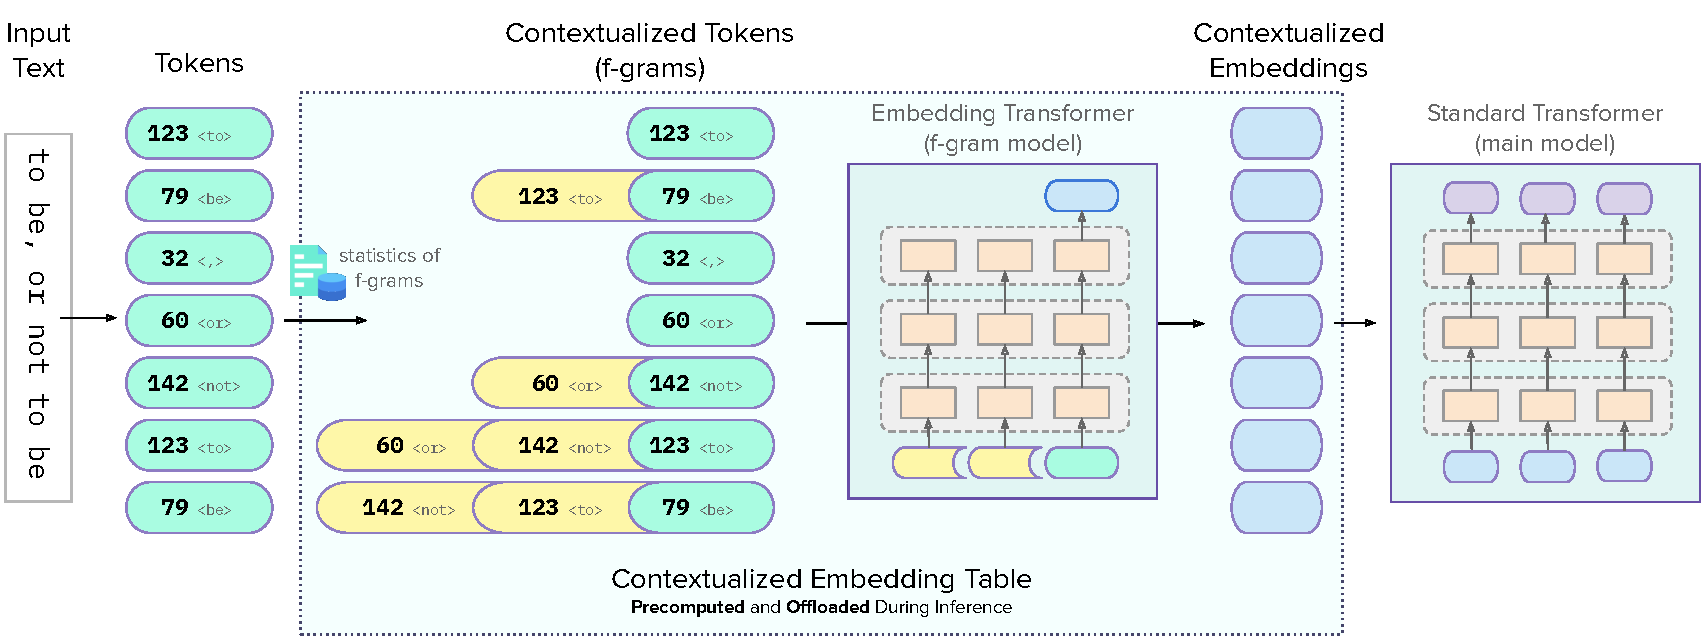
\includegraphics[width=.95\linewidth]{figs/ngram-embedding-illustration.pdf}
    \caption{Illustration of \SCONE with a maximum \ngram{n} length of 3. The {\em f-grams} are a set of frequent \ngram{n}s selected using the method described in \Cref{subsec:key_discovery}.}
    \label{fig:method_overview}
\end{figure*}

However, scaling the embedding layer by simply increasing the token vocabulary size has limited benefits. A larger vocabulary also enlarges the output (logits) layer, whose weight matrix is tied to the vocabulary size and embedding dimension. Typically, predicting the next token requires computing logits over all tokens in the vocabulary, and prior work shows that the decoding cost becomes impractical once the vocabulary exceeds a few hundred thousand tokens \citep{wang2019improving, zheng2021allocating, liang2023xlm, tao2024scaling, dagan2024getting}. Even if faster hardware or more efficient algorithms might partially offset this cost \citep{joulin2017efficient, shim2017svd}, a second problem remains: scaling the token vocabulary leads to a large number of \emph{tail tokens}, which occur infrequently in the training corpus. The embeddings of these tokens (both input and output) receive very few updates, resulting in lower-quality representations \citep{liao2021efficient, dou2024sailor}. In \Cref{sec:scale_vocab}, we train GPT-2 models with vocabulary sizes ranging from 32K to 2M and observe performance degradation as the vocabulary size exceeds 512K. We attribute this degradation to the increasing sparsity of updates per token as the vocabulary grows. Additionally, we observe a linear increase in accelerator memory usage once the vocabulary size exceeds 1M.

\noindent\textbf{Our contributions.} In this paper, we propose \SCONE, a novel approach for scaling input embedding layers by learning them through a separate transformer model, referred to as the \emph{f-gram model}. This model takes as input a set of frequently occurring \ngram{n}s (called \emph{f-grams}), which we select using an approach inspired by Byte-Pair Encoding-based tokenization (\Cref{subsec:key_discovery}). Crucially, the number of f-grams is decoupled from the token vocabulary size, allowing us to build a separate f-gram input embedding table with up to billions of entries, without blowing up the vocabulary size. An overview of the proposed method is illustrated in \Cref{fig:method_overview}.

During both training and inference, \SCONE leverages the f-gram model to efficiently handle large embedding spaces without overwhelming accelerator resources. During training, the f-gram model learns to generate contextualized embeddings for each f-gram without requiring the instantiation of a massive embedding table.  During inference, the output of the f-gram model can be precomputed to form the \emph{f-gram embedding layer}. This embedding layer can then be offloaded from the accelerator, thereby eliminating the need for accelerator resources during inference.

\SCONE introduces two novel scaling approaches for improving model performance: (i) increasing the number of cached f-gram embeddings and (ii) scaling up the f-gram model used to learn these embeddings. The first approach requires additional off-accelerator memory during inference, while the second demands greater accelerator resources during training. Importantly, both approaches preserve a fixed inference-time accelerator resource footprint, a property \emph{not}  supported by traditional scaling methods. Indeed, prior works \citep{jones2021scaling, hoffmann2022training} have shown that scaling the training compute for a fixed model size beyond some compute-optimal threshold leads to diminishing returns. Therefore, the typical method for utilizing additional training compute is to increase model size. However, directly scaling model size also increases FLOPS and accelerator memory requirements during inference. In contrast, \SCONE leverages larger f-gram models to effectively consume more accelerator resources during training but without increasing inference-time accelerator demands, offering a novel scaling paradigm that previous studies have not explored. 

There are important scenarios where maintaining a fixed inference-time accelerator footprint is especially valuable. In many deployments, where a model is queried billions of times per day, inference costs during deployment can far exceed training costs. In such cases, even small increases in inference-time computation can lead to substantial operational expenses. The recent emergence of test-time scaling techniques further highlights this trend \citep{jones2021scaling, snell2024scaling}, emphasizing situations where inference costs dominate the overall expenses of LLM deployment. Furthermore, many latency-sensitive applications impose strict limits on inference-time computation, leaving no margin for increased computational demands during deployment.

Our contributions can be summarized as follows:
\begin{itemize}[nosep,topsep=-2pt]
\item A new scalable method, \SCONE, to improve language models by expanding the input embeddings (\Cref{sec:method}) but requiring no additional accelerator resources at inference time.
\item Extensive experiments to validate \SCONE, analyzing key design choices and their impact on evaluation perplexity and accuracy on downstream tasks (\Cref{sec:exps_openwebtext}).
\end{itemize}
Our results show that \SCONE significantly boosts model performance without introducing inference latency bottlenecks; \Cref{fig:olmo_scaling_result} highlights representative findings. Notably, a \SCONE model with 1B accelerator-resident parameters outperforms a 1.9B baseline that requires approximately 2$\times$ more inference FLOPS and accelerator memory.


\begin{figure}[t]
    \centering
    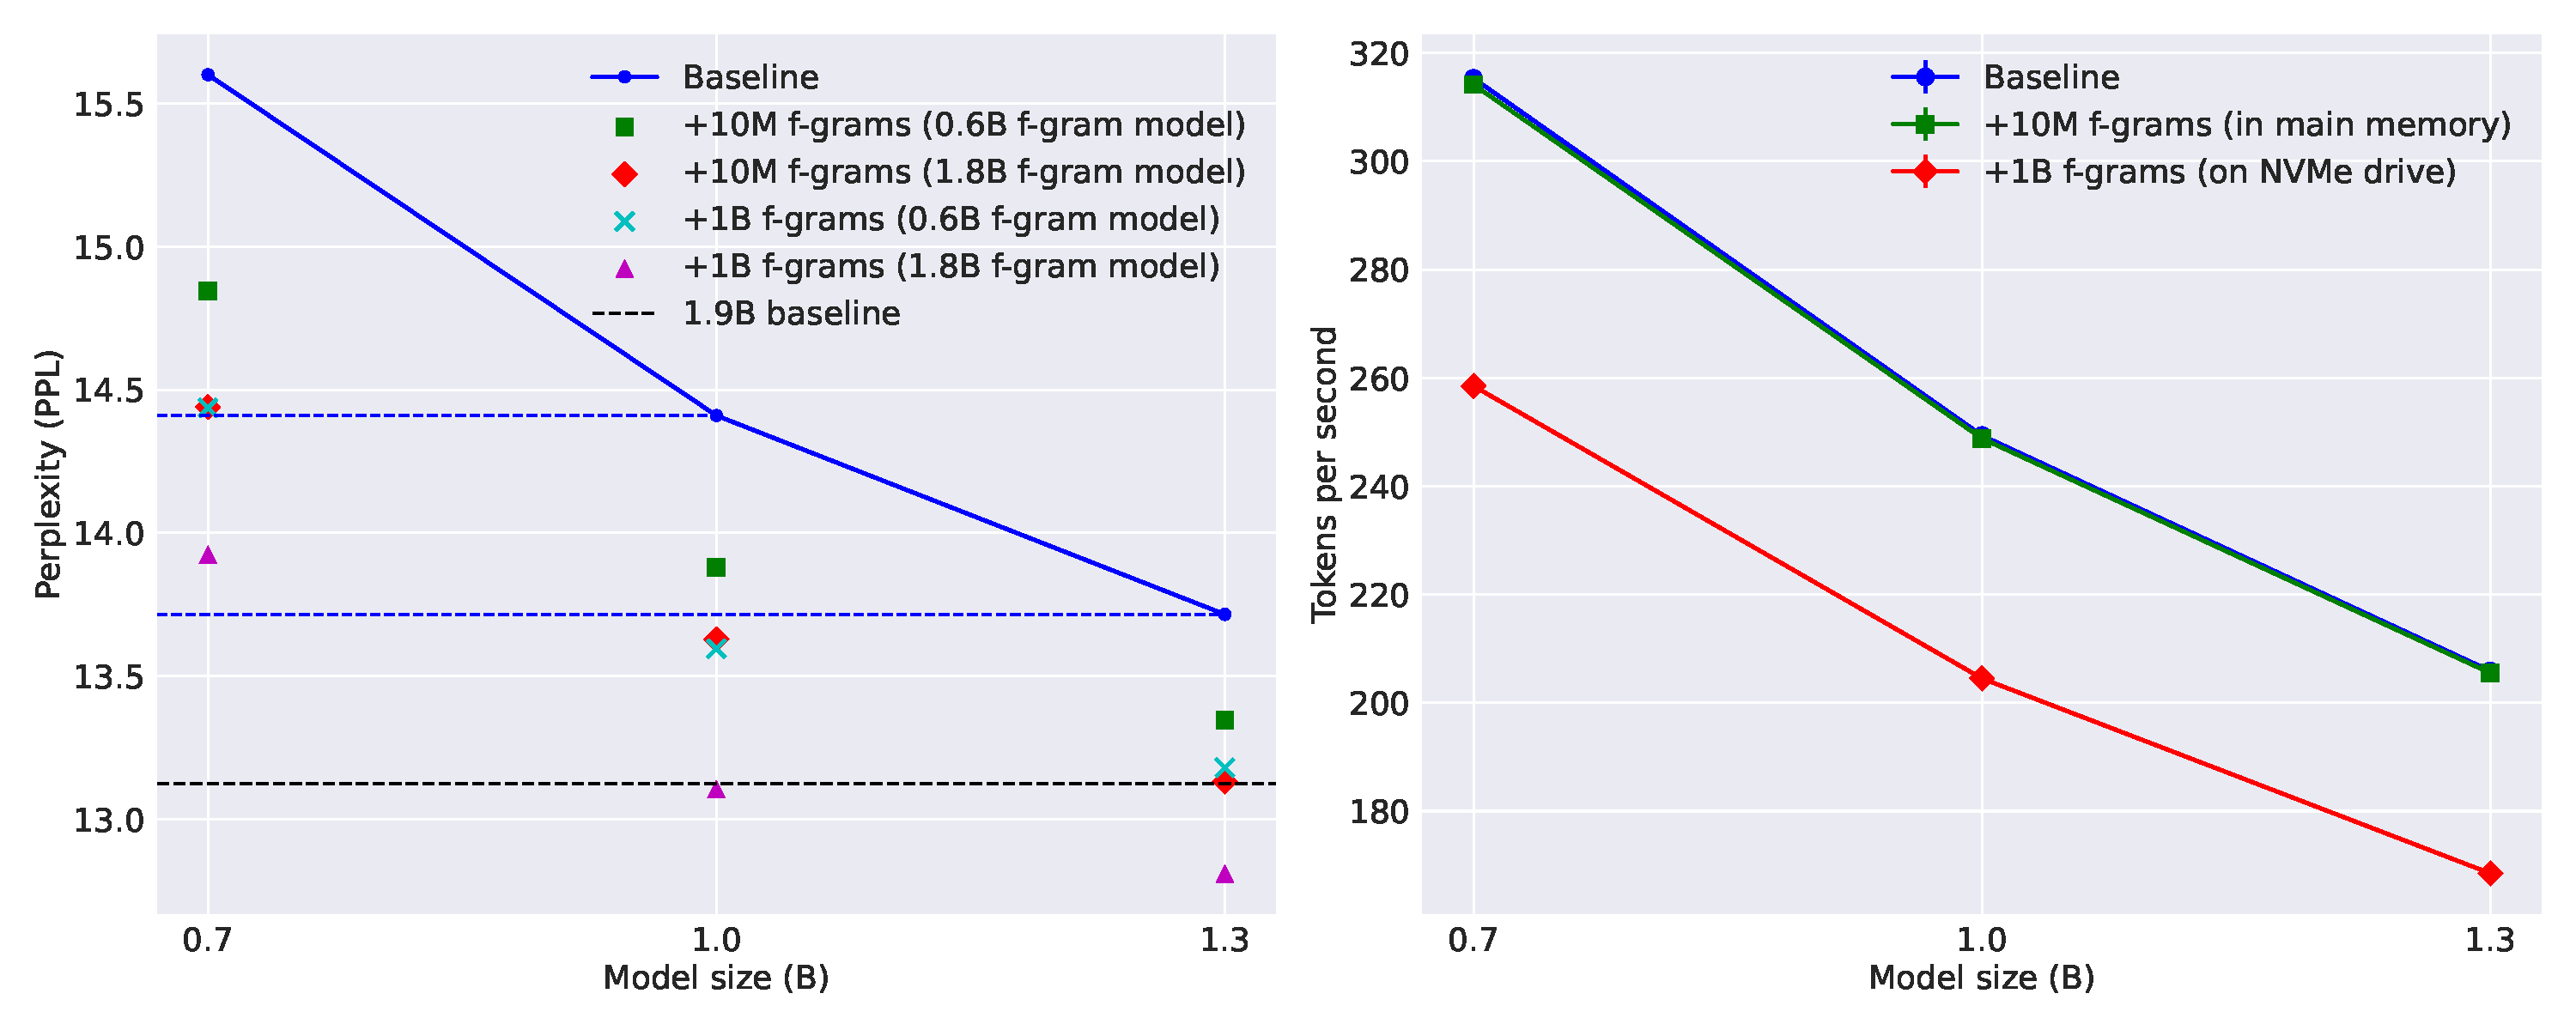
\includegraphics[width=0.8\linewidth]{figs/olmo_headline.pdf}
    \caption{\small  \textbf{(Left)} Perplexity on the OLMo \citep{OLMo} evaluation set. Model sizes along the $x$-axis indicate the number of parameters residing on the accelerator during inference.  With 10M f-grams, the 1.3B model matches the performance of the 1.9B baseline; with 1B f-grams, the 1B model surpasses it. \textbf{(Right)} End-to-end token generation speed on a single A100 GPU. Storing f-gram embeddings in main memory adds negligible latency, while using NVMe storage introduces a minor slowdown without causing a bottleneck.}
    \label{fig:olmo_scaling_result}
\end{figure}